% Standalone version of the report's methodology diagram (Fig.~3.2), rendered
% to poster/figures/methodology.png for the poster. Keep in sync with the
% tikzpicture in report/chapters/03_methodology.tex.
% Build: pdflatex methodology_standalone.tex && pdftoppm -png -r 300 \
%        methodology_standalone.pdf methodology && mv methodology-1.png methodology.png
\documentclass[border=8pt]{standalone}
\usepackage{tikz}
\usetikzlibrary{arrows.meta, positioning, calc}
\begin{document}
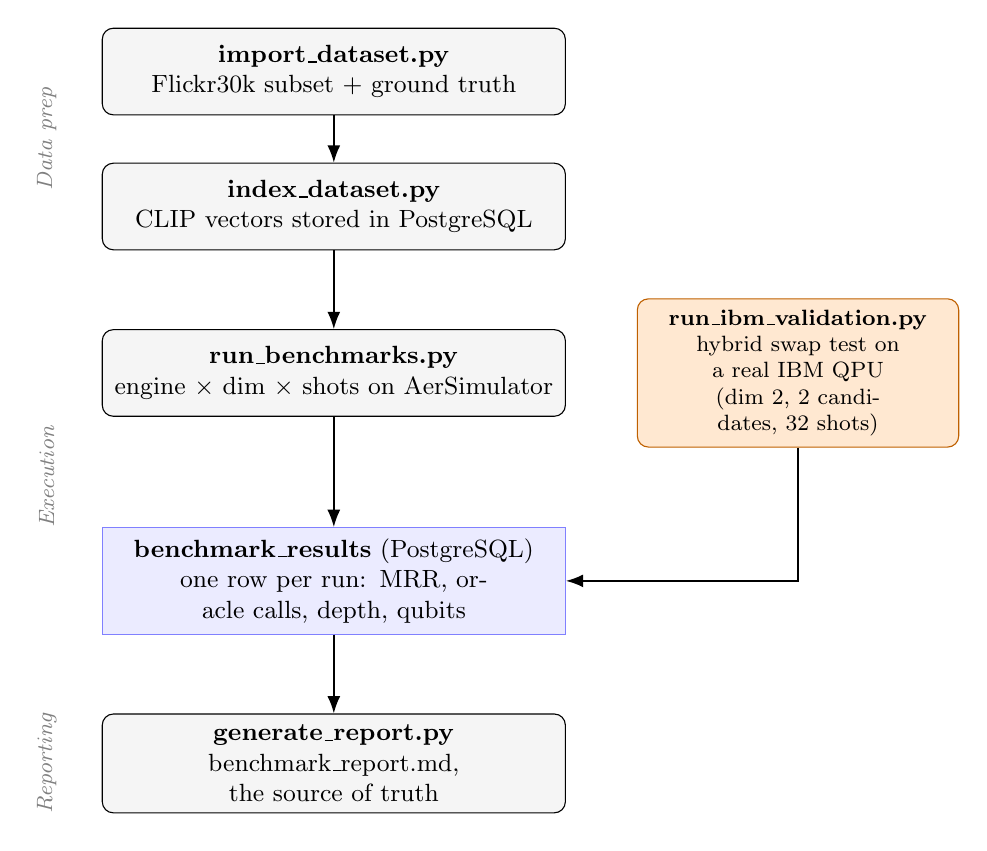
\begin{tikzpicture}[
    font=\small,
    procbox/.style={draw, rounded corners, align=center, inner sep=4pt,
      text width=56mm, fill=gray!8, minimum height=11mm},
    store/.style={draw, align=center, inner sep=4pt, text width=56mm,
      fill=blue!8, draw=blue!50, minimum height=10mm},
    ibm/.style={draw, rounded corners, align=center, inner sep=4pt,
      text width=38mm, fill=orange!18, draw=orange!75!black,
      minimum height=16mm, font=\footnotesize},
    lane/.style={font=\footnotesize\itshape, text=gray, rotate=90},
    arr/.style={-{Latex[length=2.2mm]}, semithick}
  ]
  \node[procbox] (imp) {\textbf{import\_dataset.py}\\ Flickr30k subset + ground truth};
  \node[procbox, below=6mm of imp] (idx) {\textbf{index\_dataset.py}\\ CLIP vectors stored in PostgreSQL};
  \node[procbox, below=10mm of idx] (run) {\textbf{run\_benchmarks.py}\\ engine $\times$ dim $\times$ shots on AerSimulator};
  \node[store, below=14mm of run] (res) {\textbf{benchmark\_results} (PostgreSQL)\\ one row per run: MRR, oracle calls, depth, qubits};
  \node[procbox, below=10mm of res] (rep) {\textbf{generate\_report.py}\\ benchmark\_report.md, the source of truth};

  \node[ibm, right=9mm of run] (ibm) {\textbf{run\_ibm\_validation.py}\\ hybrid swap test on a real IBM QPU\\ (dim 2, 2 candidates, 32 shots)};

  \node[lane] at ([xshift=-7mm]$(imp.west)!0.5!(idx.west)$) {Data prep};
  \node[lane] at ([xshift=-7mm]$(run.west)!0.5!(res.west)$) {Execution};
  \node[lane] at ([xshift=-7mm]rep.west) {Reporting};

  \draw[arr] (imp) -- (idx);
  \draw[arr] (idx) -- (run);
  \draw[arr] (run) -- (res);
  \draw[arr] (res) -- (rep);
  \draw[arr] (ibm.south) |- (res.east);
\end{tikzpicture}
\end{document}
